
\section{ARIMA}

Per prima cosa è stata analizzata la stazionarietà. È stata osservata una correlazione lineare tra varianza e media a diversi mesi, con R=0.86 e p-value=0.0003, suggerendo l'utilizzo del logaritmo sulla serie. Il test di Augmented Dickey-Fuller, con un p-value di 0.20, conferma inoltre che la serie non è stazionaria in media, e necessita di una differenziazione. 

\begin{figure}[H]
\centering
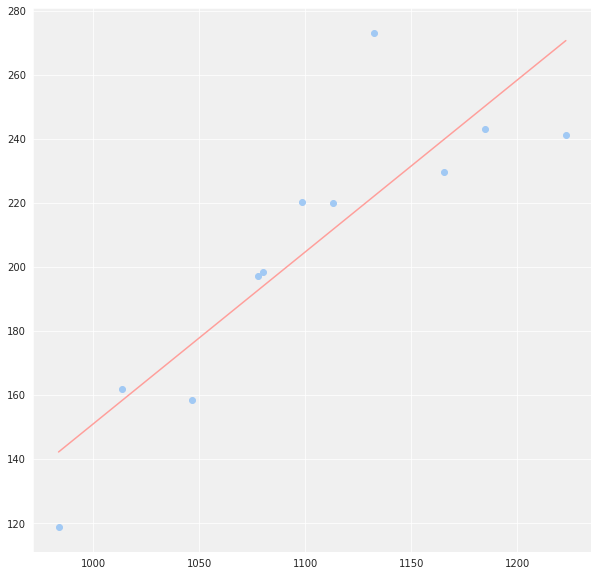
\includegraphics[width=7cm]{Pictures/medie_varianze.png}
\caption{Correlazione lineare tra varianze e medie.}
\end{figure}

Osservando invece i grafici ACF e PACF della serie iniziale, si nota una chiara stagionalità ogni 24 osservazioni (1 giorno), come già notato nella fase iniziale di esplorazione del dataset. 

\begin{figure}[H]
\centering
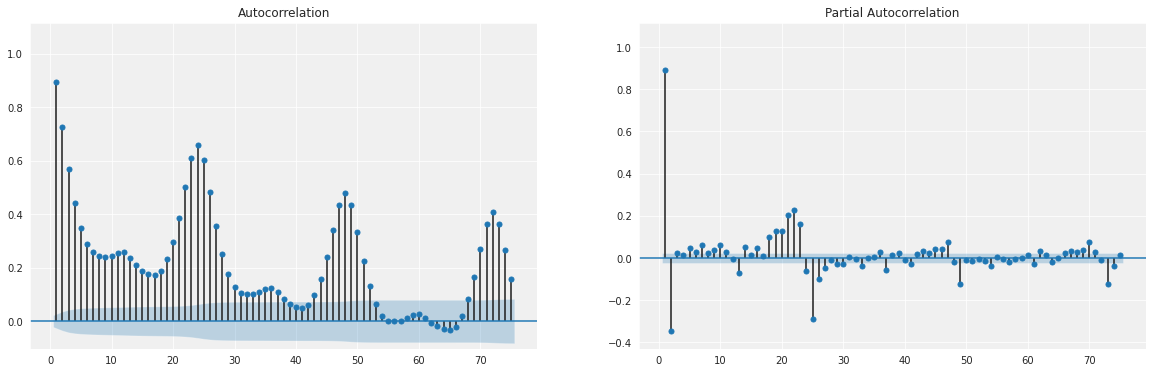
\includegraphics[width=13cm]{Pictures/acf_pacf_1.png}
\caption{ACF e PACF iniziali.}
\end{figure}

Di conseguenza, è stato creato un primo modello, sul logaritmo della serie storica: $ARIMA (0,1,0) (0,1,0) [24]$. Analizzando i suoi residui, si nota come sia necessaria l'aggiunta di un $SMA(1)$, come di solito accade differenziando. 

Viene costruito quindi il modello: $ARIMA (0,1,0) (0,1,1) [24]$. I suoi residui sono migliorati, avendo valori più contenuti nelle bande di confidenza, ma rimane della non stocasticità nei residui stagionali giornalieri. Purtroppo, non è stato individuato un modo per ridurli ulteriormente. Il MAPE sul validation set ha un valore di 11.87\%, mentre un AIC di -19660. 

\begin{figure}[H]
\centering
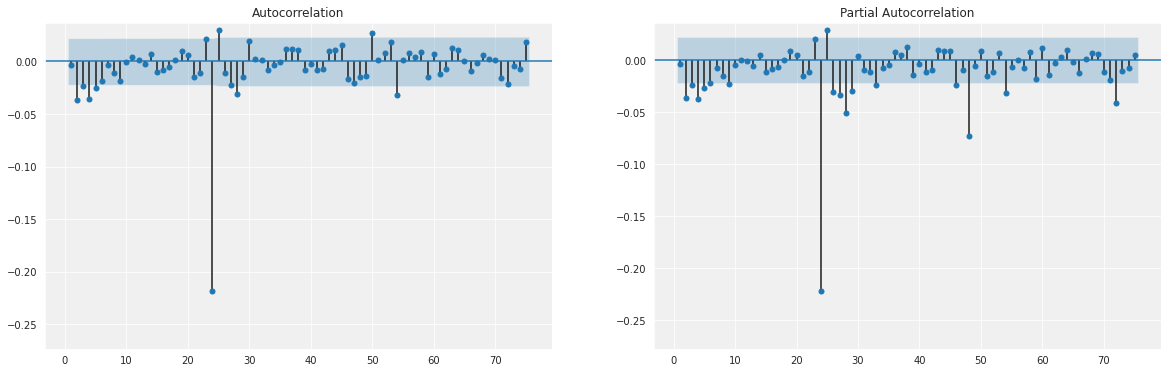
\includegraphics[width=13cm]{Pictures/acf_pacf_2.png}
\caption{ACF e PACF dei residui del modello $ARIMA (0,1,0) (0,1,1) [24]$.}
\end{figure}

Per quanto riguarda i residui a lag inferori, non stagionali, essi non sono direttamente interpretabili a dei valori di $p$ e $q$. Per questo, è stata fatta una grid-search per trovare il modello che modellasse meglio i dati, in termini di AIC e MAPE. I valori risultanti sono $p=2$ e $q=2$, con un MAPE di 11.52\% e un AIC di -20212. 

Si giunge quindi al modello: $ARIMA (2,1,2) (0,1,1) [24]$. Rimane ancora da modellare la stagionalità settimanale, chiaramente visibile nei grafici ACF e PACF a lag più alti. Questa viene modellata utilizzando delle sinusoidi, a periodo 168. 

\begin{figure}[H]
\centering
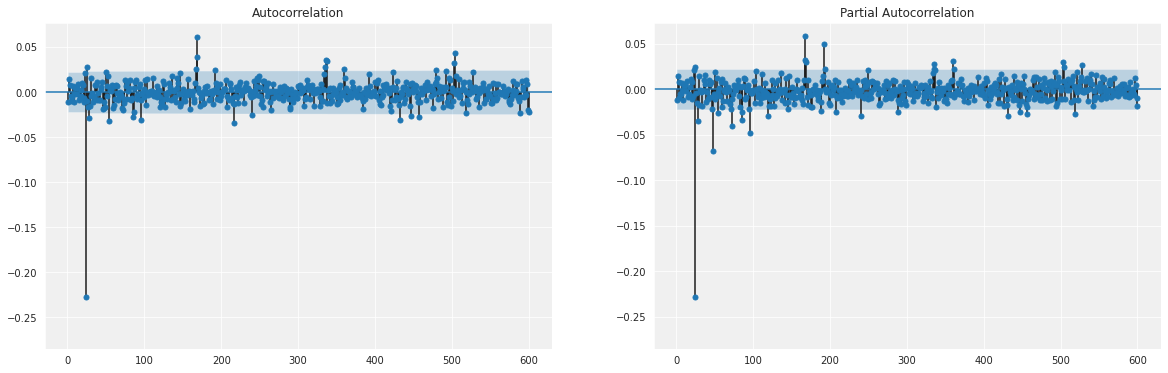
\includegraphics[width=13cm]{Pictures/acf_pacf_3.png}
\caption{ACF e PACF dei residui del modello $ARIMA (2,1,2) (0,1,1) [24]$, questa volta a 600 lag.}
\end{figure}

Dopo un test per verificare quale fosse il numero ottimale di sinusoidi, ovvero 3, è stato creato il modello. Di nuovo, c'è un miglioramento dell'AIC a -20249 e del MAPE sul validation set a 10.94\%. 

Un'ultima versione consiste nell'aggiungere dei regressori dummy per modellare le festività, le quali possono avere dei valori anomali. Dopo un'analisi (manuale) sulla serie storica, si è notato come in poche di essere si verificano eventi fuori dal comune, come il 25 aprile, 2 giugno, 25 dicembre, ecc. Il loro inserimento, in realtà, non comporta miglioramenti in termini di MAPE e di AIC. 

In conclusione, il miglior modello ARIMA presenta un AIC di -20249 e un MAPE di 10.94\%. 

\begin{figure}[H]
\centering
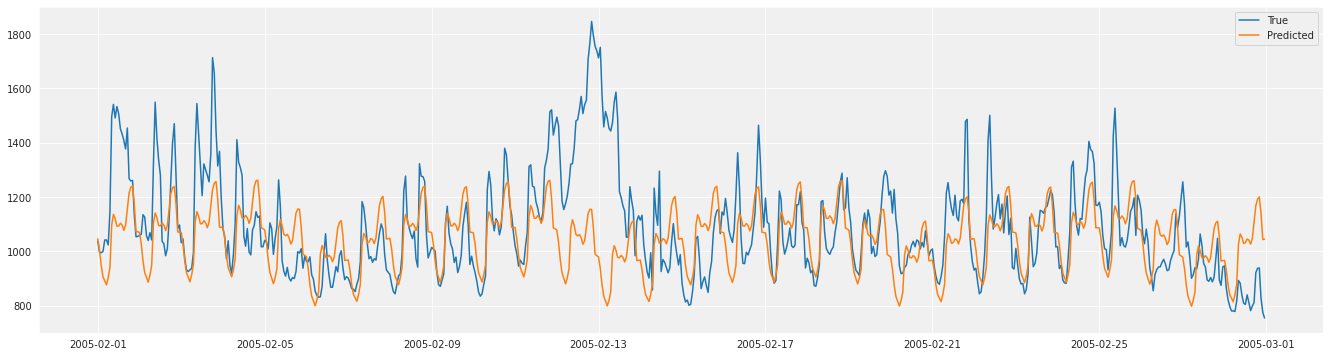
\includegraphics[width=14cm]{Pictures/prediction_arima.png}
\caption{Previsione finale del modello ARIMA.}
\label{plot_arima}
\end{figure}

Dalla figura \ref{plot_arima} si può notare come la stagionalità settimanale sia perfettamente catturata, un po' meno la giornaliera, che è meno stabile nel tempo. Inoltre, i valori anormali del 12-13 febbraio non vengono catturati. 

Infine, individuato il modello più performante, viene verificato che i suoi residui siano generati da un processo white noise, quindi a media nulla, varianza costante e incorrelati con il proprio passato. Mentre i primi due criteri vengono rispettati, l'ultimo non completamente; rimane, infatti, della memoria significativa non modellata. Questo può anche essere causato dal fatto che, trattandosi di dati reali, è difficile ottenere dei residui white noise perfetti.

\vspace{0.5cm}

\begin{figure}[H]
\centering
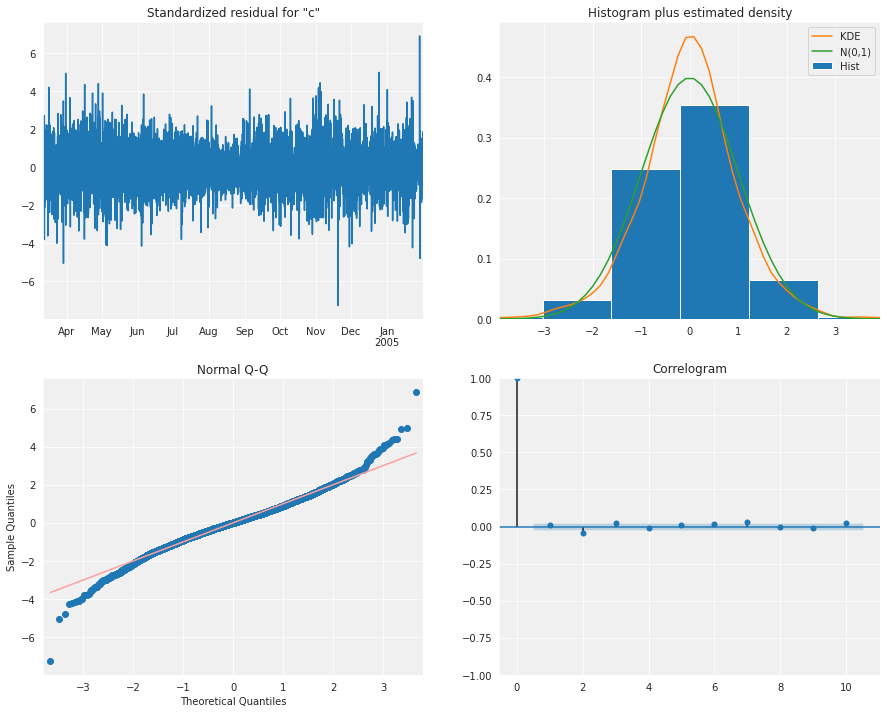
\includegraphics[width=12cm]{Pictures/summary_arima.png}
\caption{Riepilogo sui residui del modello.}
\end{figure}

